\documentclass[11pt]{article}
\usepackage[margin=0.86in]{geometry}
\usepackage{amsmath,amssymb}
\usepackage{booktabs,longtable,array}
\usepackage{graphicx}
\usepackage{microtype}
\usepackage{natbib}
\usepackage[hidelinks]{hyperref}
\usepackage{xcolor}
\usepackage{lineno}
\usepackage{authblk}

\graphicspath{{figures/}}
\linenumbers

\title{\textbf{Reconstructing a Weak-Lensing Radial-Acceleration Relation from Public Object-Level Data:}\\
Spin-2 Orientation, Additive-Control Contamination, and a Paired-Covariance Gate}
\author[1]{Facundo Firmenich}
\affil[1]{Centro de Estudios del Sur (CEDESUR), Universidad Nacional Arturo Jauretche, Buenos Aires, Argentina}
\date{Working manuscript --- evidence cut 2026-10-30}

\begin{document}
\maketitle

\begin{abstract}
Independent reconstruction of weak-lensing radial-acceleration relations (RARs)
requires more than reproducing a published curve: the lens selection, spin-2
orientation, source--lens pairing, random-centre subtraction, deprojection, and
covariance must share one auditable estimator. We report an object-level
reconstruction built from public KiDS-1000 products. The pipeline scans
21,262,011 source rows, exactly recovers the declared 106,843-lens selection,
and accumulates 3,017,858,899 accepted source--lens pairs. A preregistered
four-convention diagnostic localizes the dominant historical discrepancy to
the catalogue $e_2$ sign convention in the right-ascension/declination frame.
The corrected estimator reduces the median absolute log discrepancy from
1.03654 to 0.04943 dex, retains 15/15 positive RAR bins, and keeps the largest
cross-channel residual below 1.76 diagonal standard deviations. It nevertheless
fails the frozen reproduction gate because only 10/15 deproject-first central
values lie within the published total $1\sigma$ envelopes. A real stratified
pilot using 10,060 random centres and 433,841,322 accepted pairs finds a
material large-scale tangential control; in the outermost bin its subtraction
changes the inferred sign. The pilot cannot replace the frozen 45,038,900-centre
control. We therefore formalize the next estimand as $D=S-R$ with matched
delete-one spatial replicates and covariance
$C_D=C_S+C_R-C_{SR}-C_{SR}^{\mathsf T}$. The present result is an estimator
audit and replication boundary, not a dark-matter, modified-gravity, or plasma
detection.
\end{abstract}

\noindent\textbf{Keywords:} weak gravitational lensing; galaxy--galaxy
lensing; radial acceleration relation; reproducibility; covariance; survey
systematics

\section{Introduction}

Galaxy--galaxy weak lensing measures the coherent distortion of background
source shapes around a foreground lens population. At the required precision,
the observable is inseparable from source calibration, angular conventions,
survey geometry, redshift weighting, additive controls, and covariance
construction \citep{Mandelbaum2018,Singh2017}. Radial-acceleration relations
extend this inference by converting an excess-surface-density profile into an
effective radial acceleration and comparing it with the acceleration predicted
from baryonic mass.

KiDS-1000 has supplied both public weak-lensing products and published RAR
analyses \citep{Kuijken2019,Wright2020,Brouwer2021}. A later joint
kinematic--lensing analysis introduced an exact deprojection formula and
reported a smooth continuation of the kinematic RAR over roughly 2.5 dex in
acceleration \citep{Mistele2024}. These results motivate a demanding
reproducibility question: can the RAR be reconstructed from public object-level
inputs without importing the target curve into the estimator?

The contribution here is not a new physical ontology for the mass discrepancy.
It is a staged reconstruction in which adverse results are retained. The
pipeline first establishes byte-level custody and exact sample selection, then
executes the full source--lens accumulation, diagnoses orientation with rules
fixed before comparing the four candidates, measures a real random-centre
pilot, and finally freezes the paired-covariance gate required for a corrected
RAR. This separation prevents successful software tests or a visually similar
curve from being relabelled as physical confirmation.

\section{Data and jurisdiction}

\subsection{Public source and lens products}

The source surface is the KiDS-1000 SOM-gold weak-lensing catalogue. Its
17,712,469,440 bytes are represented by 185 contiguous remote byte ranges so
that the full file need not be materialized on a workstation. The complete
scan covers 21,262,011 rows. Published quality cuts retain 19,109,925 rows with
finite positive shape weights. The five photometric-bin counts are
1,727,608; 3,442,980; 5,624,220; 4,006,695; and 4,308,422.

Native GAAP $u$- and $r$-band photometry was aligned object by object for
1,239,422 KiDS-bright records. Applying the declared isolation and selection
geometry exactly recovers 106,843 lenses, with zero count difference and no
reconstructed-magnitude fallback. The official five SOM $n(z)$ distributions
were integrated behind the lens posterior to form an effective critical
surface-density lookup spanning
$3.047\times10^{15}$--$9.010\times10^{15}\,M_\odot\,\mathrm{Mpc}^{-2}$.

\subsection{Stage authority}

Table~\ref{tab:authority} records what each completed stage can establish. A
stage may validate an input or estimator while remaining explicitly
non-authoritative for a physical claim.

\begin{table}[ht]
\centering
\caption{Authority of the executed reconstruction stages.}
\label{tab:authority}
\small
\begin{tabular}{p{0.19\linewidth}p{0.34\linewidth}p{0.34\linewidth}}
\toprule
Stage & Completed evidence & Claim not licensed \\
\midrule
v0.16 & Exact lens selection; full source attrition; published-bin RAR transform & Object-level lensing reproduction or mechanism \\
v0.17 signal & 21.26 million sources, 106,843 lenses, 3.018 billion accepted pairs & Corrected survey estimator without random subtraction \\
v0.17 orientation & Frozen comparison of four spin-2 conventions & Final reproduction or model selection \\
v0.17 random pilot & 10,060 real random centres; 433.84 million accepted pairs & Frozen 45.04 million-centre control \\
v0.18 gate & Input integrity and paired-covariance implementation tests & New corrected RAR or scientific success \\
\bottomrule
\end{tabular}
\end{table}

\section{Estimator}

\subsection{Spin-2 rotation}

For a source ellipticity $(e_1,e_2)$ and a source--lens polar angle $\phi$
measured from east, the repaired KiDS right-ascension/declination convention is
\begin{align}
e_t &= -\left[e_1\cos(2\phi)-e_2\sin(2\phi)\right],\\
e_\times &= e_1\sin(2\phi)+e_2\cos(2\phi).
\end{align}
The four-candidate diagnostic crossed two angular origins with the documented
$e_2$ sign transformation. Candidate definitions, the pass rule, and the
published comparison were frozen before adjudication. The implementation
retains the four linear basis accumulators, so conventions can be evaluated
without rereading the 17.7 GB source surface or adaptively rotating the data.

\subsection{From excess surface density to acceleration}

Each accepted lens--source pair contributes weighted sufficient statistics in
27 projected-radius bins. Source redshift uncertainty enters through the
effective critical surface density. The deproject-first channel applies the
signed linear deprojection operator to each lens profile before stacking,
following the exact transformation in \citet{Mistele2024}; it is kept distinct
from a stack-first singular-isothermal-sphere diagnostic.

The full signal scan was split into eight contiguous source-row partitions.
Every partition preserves the lens payload, radial edges, and critical-density
lookup hashes. The merged artifact covers $[0,21{,}262{,}011)$ without a gap
and has content SHA-256 prefix \texttt{5d5f8c3a11cbe99b}; the complete
digest is retained in the evidence ledger distributed with the package.

\subsection{Corrected estimand and covariance}

Let $S$ denote the signal-centre estimator and $R$ the random-centre estimator.
The survey-corrected quantity is
\begin{equation}
D=S-R.
\end{equation}
If both populations reuse source galaxies, independence cannot be assumed.
Matched spatial delete-one replicates give
\begin{equation}
C_D=C_S+C_R-C_{SR}-C_{SR}^{\mathsf T}.
\label{eq:pairedcov}
\end{equation}
The implementation operates on region-level additive sufficient sums, deletes
the same region from $S$ and $R$, and builds one joint vector containing
tangential, cross, deproject-first tangential, and deproject-first cross
channels. A coordinate is estimable only when finite in the full estimator and
every matched replicate. Pairwise deletion, zero filling, diagonal
substitution, automatic inversion, and a silent Hartlap correction
\citep{Hartlap2007} are prohibited.

\section{Results}

\subsection{Full object-level signal scan}

The complete eight-partition scan evaluates all 21,262,011 source rows against
the exact 106,843-lens payload and accepts 3,017,858,899 pairs. The merged
sufficient-statistics surface is compact (138.6 MB across the eight sealed
artifacts) because individual pairs are never persisted. Continuous row
coverage and content hashes separate the observational result from transport
and reporting failures.

\subsection{Orientation repair}

Figure~\ref{fig:orientation} shows the only preregistered repair candidate. The
catalogue-$e_2$ sign transformation reduces the deproject-first median absolute
log discrepancy from 1.0365400070 to 0.0494255413 dex, an improvement of
0.9871144657 dex. All 15 central values are positive, and the largest
cross-channel residual is 1.75594 diagonal standard deviations. The independent
stack-first diagnostic gives a 0.0436427705 dex median discrepancy and 15/15
positive bins.

\begin{figure}[ht]
\centering
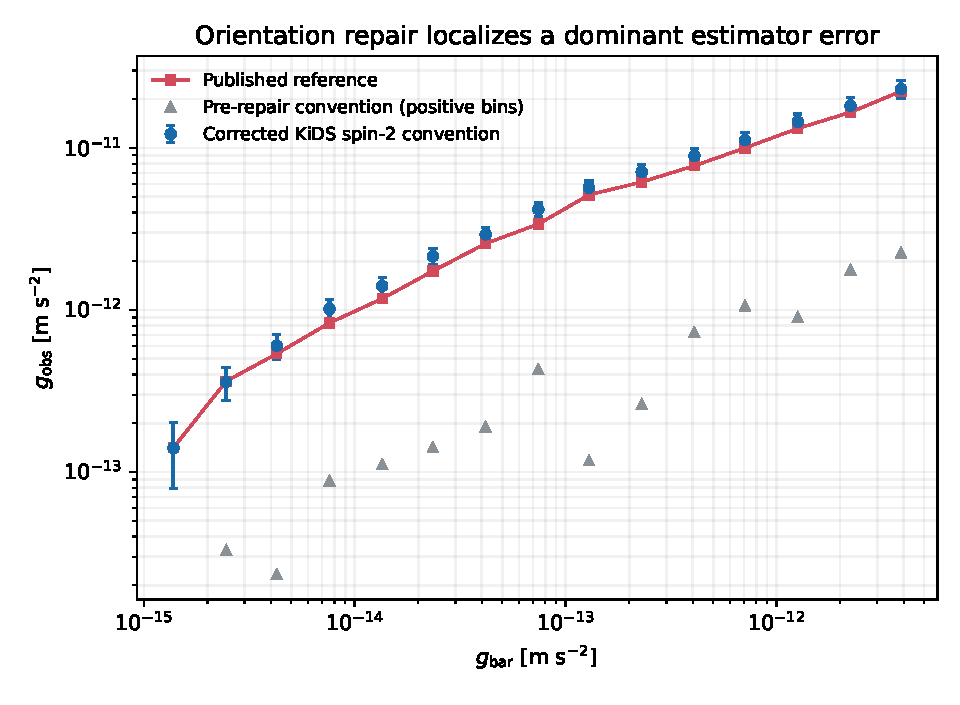
\includegraphics[width=0.79\linewidth]{darkpipe_orientation_repair.pdf}
\caption{Object-level RAR after the frozen spin-2 orientation adjudication.
Error bars are the available diagonal uncertainties; they are not a substitute
for the paired spatial covariance in Eq.~\eqref{eq:pairedcov}.}
\label{fig:orientation}
\end{figure}

The repair is substantial but not a completed reproduction. Only 10/15
deproject-first central values and 12/15 stack-first values fall within the
published total $1\sigma$ envelopes. The frozen rule therefore returns
\texttt{reproduction\_gate=false}. That adverse decision is preserved rather
than weakening the threshold after seeing the improved curve.

\subsection{A real random-centre pilot}

The random pilot uses ten positions in each of the 1,006 official survey tiles,
for 10,060 centres total. Against the same 21,262,011-source surface, it
evaluates 575,059,669 candidate pairs and accepts 433,841,322. The largest
cross-channel diagnostic stays below 1.87 diagonal standard deviations.

The tangential random surface is nevertheless material. At
$R=10.24094\,h_{70}^{-1}\,\mathrm{Mpc}$,
\begin{align}
\Delta\Sigma_R &=(-2.8076\pm0.9209)\times10^{11}
\,M_\odot\,\mathrm{Mpc}^{-2},\\
g_{\mathrm{obs},R} &=(-1.5591\pm0.3120)\times10^{-13}
\,\mathrm{m\,s^{-2}},
\end{align}
using diagonal errors. These are localization diagnostics, not global
significances. At the same radius, subtracting the pilot from the signal moves
$g_{\mathrm{obs}}$ from $-5.40\times10^{-14}$ to
$+1.02\times10^{-13}\,\mathrm{m\,s^{-2}}$.

\begin{figure}[ht]
\centering
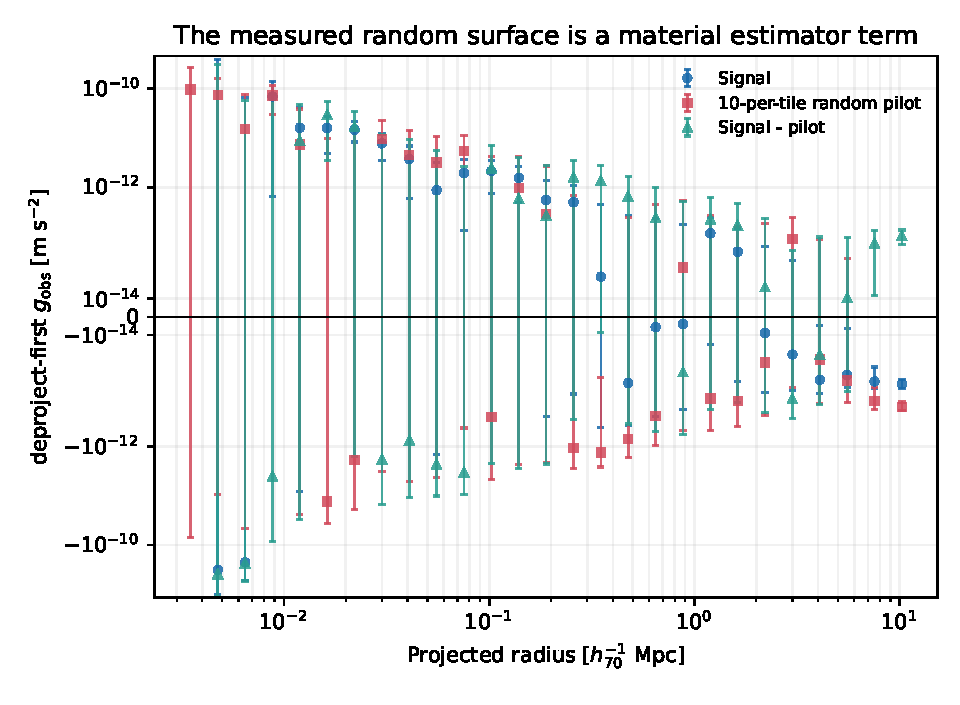
\includegraphics[width=0.79\linewidth]{darkpipe_random_control.pdf}
\caption{Full signal, measured stratified random pilot, and their exploratory
difference. The signed logarithmic ordinate preserves negative values. The
pilot demonstrates estimator materiality but cannot replace the frozen 50x
control.}
\label{fig:random}
\end{figure}

\subsection{Why the result stops here}

The frozen random catalogue contains 45,038,900 positions, 4,477.03 times the
pilot count. Linear extrapolation from the original implementation projects
roughly $2.57\times10^{12}$ candidate and $1.94\times10^{12}$ accepted pairs,
with 231--417 CPU hours per original partition. This estimate is a planning
bound, not a benchmark of the tile-local successor.

The v0.18 input audit passes all four frozen-file hashes, exact coverage of
21,262,011 source rows, 988 source pointings, 1,006 random tiles, and
45,038,900 allocated random positions. Seventeen focal algebra/provenance tests
pass. The terminal status remains
\texttt{BLOCKED\_EXECUTION\_AND\_PAIRED\_COVARIANCE} because the full control,
matched signal/random spatial replicates, and an admitted finite compute budget
do not yet exist.

\section{Interpretation and limits}

Three conclusions are supported. First, a sign convention in a spin-2
observable can dominate a full-catalogue reproduction while leaving transport,
selection, and deprojection machinery internally consistent. Second, the
measured random-centre surface is not a cosmetic correction: at large radius it
is comparable to or larger than the signal and can reverse its sign. Third, a
random-only jackknife estimates $C_R$, not the covariance of $S-R$; shared
sources require the cross terms in Eq.~\eqref{eq:pairedcov}.

The current evidence does not adjudicate $\Lambda$CDM, modified gravity, or a
plasma/morphotopological mechanism. It does not establish a final corrected
RAR, a global $p$-value, or a total-systematics covariance. Remaining
uncertainties include shear calibration, source photometric redshifts, lens
mass modelling, survey selection, deprojection tails, field variance, and the
design of comparable-area spatial exclusions. The 1,006 raw survey tiles are
not automatically valid equal-area jackknife regions.

\section{Confirmatory next experiment}

The decisive run has a fixed sequence:
\begin{enumerate}
\item bind a remote node with at least 40 GB scratch and a finite CPU-hour
budget;
\item execute a hard 30-minute tile-local benchmark and seal its
time/memory/pair/byte receipt;
\item freeze a justified spatial exclusion map and source-deletion policy;
\item accumulate both signal and all 45,038,900 random centres into the same
region-level sufficient statistics;
\item form matched replicates, $D=S-R$, and the full four-channel covariance;
\item apply the unchanged reproduction gate before any mechanism-level
interpretation.
\end{enumerate}
No step authorizes the next automatically; every result, including failure or
singular covariance, is a valid terminal scientific outcome.

\section{Conclusions}

The public-data reconstruction has crossed the expensive object-level
threshold: exact lens selection, the complete source scan, more than three
billion accepted signal pairs, a preregistered orientation repair, and a real
random-centre pilot. The repaired signal is close to the published RAR in
median log discrepancy but fails the stricter all-bin reproduction rule.

The most important empirical result is the boundary itself. A measured
large-scale random term is capable of materially changing the derived
acceleration surface, while the covariance of the corrected estimator requires
matched signal--random spatial replicates. Until the frozen 50x control and
Eq.~\eqref{eq:pairedcov} are executed, a final RAR or physical-model verdict
would outrun the data.

\section*{Data and code availability}

The executed code, frozen protocol, compact sufficient-statistics receipts, and
evidence files are versioned in the public repository
\url{https://github.com/FacundoFirmenich/darkpipe-realdata}. The governing
working branch is \path{v018-paired-random-covariance-gate} at commit
\texttt{df321b1f}; draft pull request 25
records the gate and adverse CI history. The raw KiDS products remain at their
official providers and are not duplicated in this paper package.

\section*{Acknowledgements}

This work uses public KiDS-1000 products. Any submitted version must include
the complete KiDS acknowledgement and programme identifiers required by the
data provider, together with the final funding, conflict, CRediT, ORCID, and
AI-assistance declarations approved by the author.

\bibliographystyle{plainnat}
\bibliography{references}

\appendix
\section{Compact evidence ledger}

\begin{longtable}{p{0.28\linewidth}p{0.18\linewidth}p{0.42\linewidth}}
\toprule
Artifact & Git blob SHA & Governing content \\
\midrule
\endhead
V016 critical checkpoint &
\texttt{a07fe9d6...} & Exact 106,843-lens closure; 21,262,011-source scan; effective critical-density lookup.\\
Orientation metrics &
\texttt{b8097436...} & Four frozen conventions; repaired median discrepancy; all-bin gate.\\
Partition custody &
\texttt{43cd6f39...} & Eight complete partitions and 3,017,858,899 accepted pairs.\\
V017 random comparison &
\texttt{7d091464...} & 10,060-centre pilot; material tangential random surface.\\
\texttt{readiness.json} &
\texttt{224855ef...} & Passing input integrity and explicit three-blocker terminal gate.\\
\bottomrule
\end{longtable}

\end{document}
